
\subsection{External Configuration  (\textit{MK})}
Many configurations of aircraft were considered during initial design phase. First, a trade study was performed over similar aircraft that are either currently in service or have flown in the past. Table \ref{tabmk1} describes seven aircraft and some of their external configuration characteristics. 

\begin{table}[H]
    \centering
    \caption{Quantitative Trade Study of Similar Aircraft}
    \begin{tabular}{|m{3cm}||c|c|c|c|c|}
    \toprule
    \label{tabmk1}
    \textbf{Aircraft} & \textbf{Tail Type} & \textbf{Wing Type} & \textbf{\# of Engines} & \textbf{2-class Seating} & \textbf{\# of Decks} \\
    \hline\hline
    Boeing 777-200 & Conventional & Low & 2 & 375 & Single \\
    \hline
    Airbus 340-600 & Conventional & Low & 4 & 440 & Single \\
    \hline
    Boeing 787-10 & Conventional & Low & 2 & 330 & Single \\
    \hline
    McDonnell Douglas MD-11 & Conventional (w/ engine) & Low & 3 & 323 & Single \\
    \hline
    Lockheed 1011-100 & Conventional (w/ engine) & Low & 3 & 304 & Single \\
    \hline
    Boeing 747-400 & Conventional & Low & 4 & 496 & Double \\
    \hline
    Airbus 350-900 & Conventional & Low & 2 & 315 & Single \\
    \bottomrule
    \end{tabular}
\end{table}

From the trade study, all seven of described aircraft featured a low-level wing along with a conventional tail. This is most likely due to the low-level wing providing space for a retractable landing gear along with simplicity of design. Thus, the has decided to go with a low-level wing.

The next external configuration decision was between a T-tail and a conventional tail. While the T-tail does reduce the risk of the tail stalling, it is much more difficult to design as the vertical tail has to support the entire weight of the horizontal tail. Alternatively, conventional tails are lighter and provide more simplicity in terms of design. Another benefit with conventional tails is that it offers more space to store fuel for the aircraft. As shown from the trade study, conventional tails are very widely used in commercial aircraft in today's market. Thus, the team decided to use a conventional tail configuration. 

\newpage

Furthermore, the number of engines on our aircraft along with the number of decks on the aircraft were to be decided. The team decided to go with a single-decker to provide simplicity in design as well reduced cost in manufacturing. Moreover, two engines were chosen for our aircraft, mainly for the reduced maintenance cost of more engines as well as a smaller fuel cost. The proven reliability of modern engines in trans-oceanic flights also played a role in deciding to have two engines. Figure \ref{fig3view} shows a top, left, front, and isometric view of the OpenVSP model of the aircraft. The Sam Mark 1 has a total length of 202 ft and a wingspan of 212 ft. 

\begin{figure}[H]
        \centering
        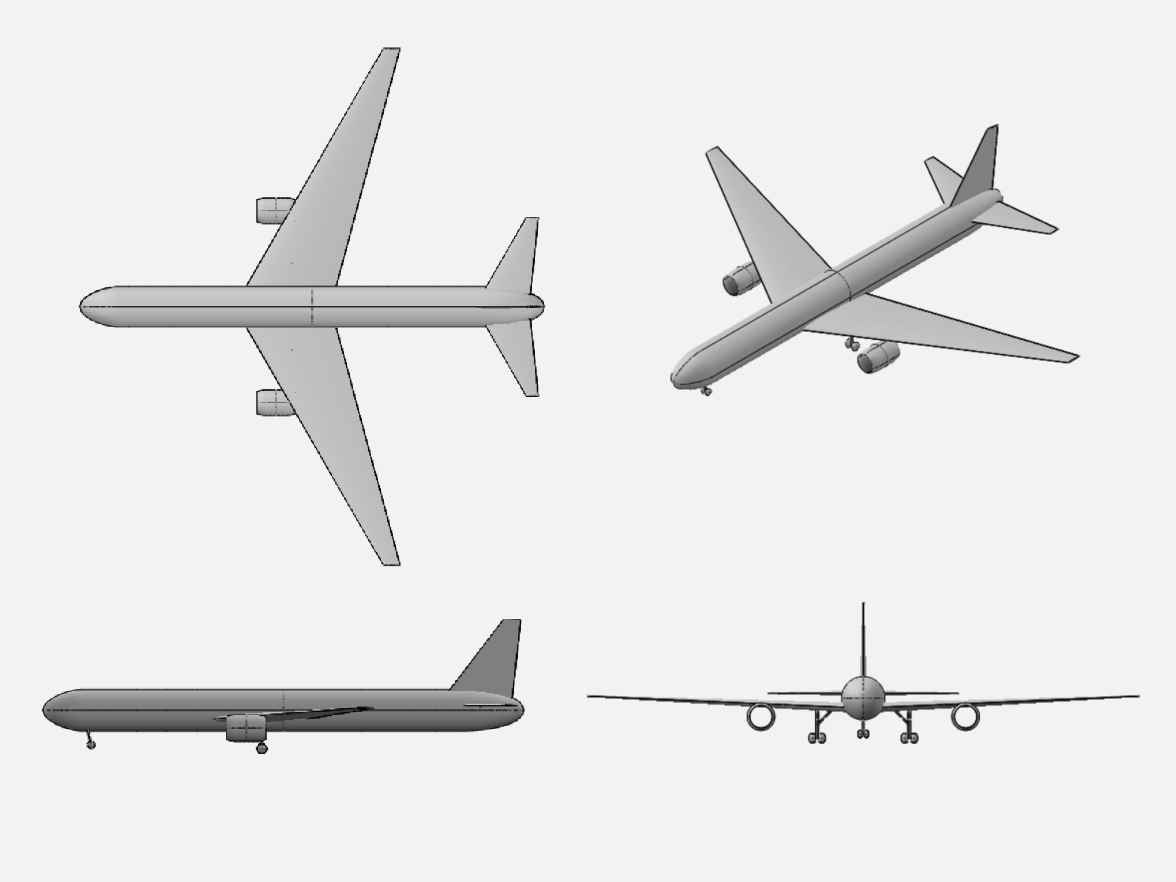
\includegraphics[width=0.75\linewidth]{Photos/3-View_Aircraft_(2-12-20).pdf}
        \caption{3-View Drawing of Sam Mark 1}
        \label{fig3view}
        \end{figure}

\subsection{Internal Configuration}
\subsubsection{Seating Configuration (\textit{JC})}
The aircraft internal configuration is a two-class seating with business and economy seating accommodations.  Per AIAA RFP requirements, the aircraft is designed with 50 business-class and 350 economy-class seats.

\begin{table}[!h]
    \centering
    \caption{Seating Configuration}
    \begin{tabular}{|c|c||c|c|} \toprule
        \multicolumn{2}{c}{\textbf{Business Class}} & \multicolumn{2}{c}{\textbf{Economy Class}} \\ \hline
        Configuration (a) & 2 - 2 - 2 & Configuration (a) & 3 - 4 - 3 \\ \hline
        Row Count (a) & 8 & Row Count (a) & 28 \\ \hline
        Configuration (b) & 1 - 0 - 1 & Configuration (b) & 2 - 3 - 2 \\ \hline
        Row Count (b) & 1 & Row Count (b) & 10 \\ \hline
        Pitch & 36" & Pitch & 32" \\ \hline
        Width & 21" & Width & 18" \\ \bottomrule
    \end{tabular}
    \label{tab:seating}
\end{table}

Two proposed seating configurations are proposed for each class above in Table \ref{tab:seating}.  The business class contains 8 rows with a 2 - 2 - 2 configuration to provide a spacious flight experience while making efficient use of the space provided.  The purpose of selecting a 2 - 2 - 2 style is to provide business passengers with aisle seating.  The 1 - 0 - 1 row is provided to accommodate ADA passengers and may be customized by the client.  The economy class has two sections with a 3 - 4 - 3 and 2 - 3 - 2 configuration.

\subsubsection{Galley Configuration}

\subsubsection{Lavatory Configuration}

\subsubsection{Door Configuration}

\hl{Include Door Certification Requirements} --> are we doing this for DRR?  @NZ



% \textcolor{red}{
% \begin{itemize}
%     \item Discuss external configuration alternatives considered and design choices made.
%     \item Discuss selected aircraft configuration design (i.e. distinctions between variants, major features, design characteristics/objectives).
%     \item Include at least one trade study that uses quantitative or qualitative analysis to support design decisions made.
%     \item Discuss the landing gear philosophy.
%     \item 3-View drawing (VSP acceptable).
%     \item Discuss future work
% \end{itemize}}